% XCircuit output "modo_discontinuo.tex" for LaTeX input from modo_discontinuo.eps
\def\putbox#1#2#3#4{\makebox[0in][l]{\makebox[#1][l]{}\raisebox{\baselineskip}[0in][0in]{\raisebox{#2}[0in][0in]{\scalebox{#3}{#4}}}}}
\def\rightbox#1{\makebox[0in][r]{#1}}
\def\centbox#1{\makebox[0in]{#1}}
\def\topbox#1{\raisebox{-0.60\baselineskip}[0in][0in]{#1}}
\def\midbox#1{\raisebox{-0.20\baselineskip}[0in][0in]{#1}}
   \scalebox{1}{
   \normalsize
   \parbox{4.46875in}{
   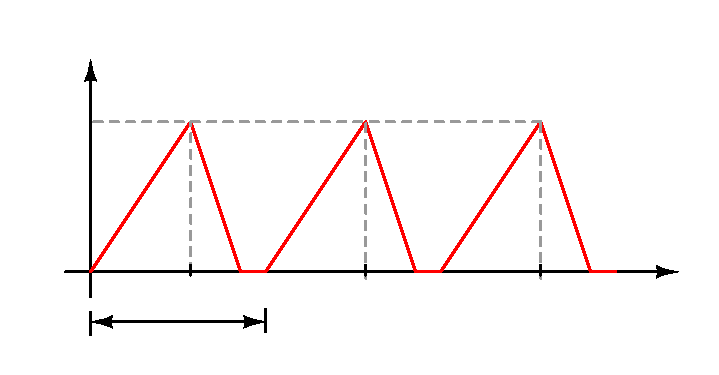
\includegraphics[scale=1]{modo_discontinuo}\\
   % translate x=756 y=228 scale 0.38
   \putbox{0.06in}{1.58in}{1.20}{$I_{Lmax}$}%
   \putbox{0.43in}{2.10in}{1.20}{$I_L$}%
   \putbox{4.45in}{0.51in}{1.20}{t}%
   \putbox{0.51in}{0.43in}{1.20}{$t_{carga}$}%
   \putbox{1.20in}{0.41in}{1.20}{$t_{des}$}%
   \putbox{1.01in}{0.06in}{1.20}{T}%
   } % close 'parbox'
   } % close 'scalebox'
   \vspace{-\baselineskip} % this is not necessary, but looks better
